

\PassOptionsToPackage{full}{textcomp}
\documentclass{tufte-handout}
%\usepackage{fontspec}
\usepackage{ETbb}

\title{Documenting Data Analysis}
\author[Barry Linkletter]{Barry Linkletter}
\date{} % without \date command, current date is supplied

%\geometry{showframe} % display margins for debugging page layout

\usepackage{graphicx} % allow embedded images
%  \setkeys{Gin}{width=\linewidth,totalheight=\textheight,keepaspectratio}
  \graphicspath{{graphics/}} % set of paths to search for images
\usepackage{amsmath}  % extended mathematics
\usepackage{booktabs} % book-quality tables
%\usepackage{units}    % non-stacked fractions and better unit spacing
\usepackage{multicol} % multiple column layout facilities
\usepackage{lipsum}   % filler text
\usepackage{fancyvrb} % extended verbatim environments
  \fvset{fontsize=\normalsize}% default font size for fancy-verbatim environments
\usepackage{gensymb} % provides symbols like \degree
\usepackage{ragged2e} % enables hyphenation in ragged-right justification
\usepackage[normalize-symbols]{textalpha} %enables \textalpha for alpha symbol etc.

\usepackage{hyperref} % enables styling of href and url
\hypersetup{
    pdftitle={Eyring Equation},
    pdfauthor={Barry Linkletter},
    colorlinks=true,
    linkcolor=blue,
    filecolor=magenta,      
    urlcolor=blue,
    pdfborder={0 0 0},
    frenchlinks=false,
    pdfpagemode=FullScreen,
    }

\usepackage{enumitem} % allows resuming enumerate lists.
\usepackage{mathtools}
\usepackage{mhchem}
\usepackage{siunitx} % provides "S" column class for aligning decimals.  
\usepackage{nicefrac}

\usepackage{varioref}

\usepackage{babel}
\usepackage{float}
\usepackage{stackrel}


\usepackage[shortconst]{physconst}

\usepackage[normalem]{ulem}  % provides strikethroul \sout{}

\begin{document}

\justifying


\maketitle% this prints the handout title, author, and date

\begin{abstract}
You have analyzed data and presented your conclusions. Can others get to the same values using your data? Could someone check your methods in detail? If you perform your analysis using \textit{Python}, the code will reveal your methods. We will explore using \textit{Python} to analyze your data in an interactive environment and to document your methodology. Along the way we will hopefully agree to never use "cubic spline" again.
\noindent \marginnote[-35mm]{This document was produced using the \LaTeX\ typesetting language with the Tufte-handout document class. Chemical diagrams were created in \textit{ChemDoodle} Plots were typeset using \textit{MatPlotLib} and \textit{Python} tools. Diagrams were created and edited using \textit{Affinity Designer}.}

\end{abstract}


\section{The Eyring Equation}

The Eyring equation is a classic of physical chemistry.\sidenote
[][-10mm]{Read chapter 7 of ``Modern Physical Organic Chemistry'' by Anslyn \& Dougherty, \textit{University Science Books}, \textbf{2006} or any textbook that discussed chemical kinetics.}
 The free energy of activation for a reaction can be determined and, if a series of rate constant values are available at different temperatures, we can determine the enthalpy and the entropy of activation. These parameters are very helpful in interpreting reaction mechanism. But can these results be trusted? How could you estimate their reliability? Unless you are calculating the standard deviations from your plot you may be unaware of a low quality relationship.

The Erying equation was developed almost 100~years ago\sidenote
[][-25mm]{"The activated complex in chemical reactions." H. Eyring,  \textit{J. Chem. Phys.}, \textbf{1935}, \textit{3}, 107-115, \url{https://doi.org/10.1063/1.1749604} \vspace{2mm}}\sidenote
[][-8mm]{"Some applications of the transition state method to the calculation of reaction velocities, especially in solution." M.G. Evans, M. Polanyi,  \textit{Trans. Faraday Soc.}, \textbf{1935}, \textit{31}, 875-894, \url{https://doi.org/10.1039/TF9353100875} \vspace{2mm}}
by Henry Eyring,\sidenote
[][0mm]{Eyring was born in Mexico in 1901 and his family fled to the USA in 1912 during the Mexican revolution. Erying was a Mormon. His father practiced polygamy and was married to the two great-aunts of former US presidential candidate Mitt Romney at the same time. You could say that Erying ``had two moms.'' He was awarded just about every honour in chemistry except the Nobel prize.\vspace{2mm}}
Michael Polanyi\sidenote
[][0mm]{Polanyi fled Germany in 1933 and was appointed a professor of physical chemistry at the University of Manchester. He was a deep thinker and was appointed to a chair in social science at U.~Manchester in 1948. He passionately argued that human nature was greater than the sum of its chemical parts. Two of his students won Nobel prizes: Eugene Wigner (a nuclear physicist who helped draft the famous "Einstein letter" that led to the creation of the atomic bomb - 1963 for physics) and Melvin Calvin (a biochemist and a leader in the elucidation of carbon fixation in photosynthesis - 1961 for chemistry.) His son, John Polanyi, is a professor emeritus of chemistry at U.~Toronto and won the Nobel prize in 1986 for chemistry. \vspace{2mm}}
and Meredith Evans.\sidenote
[][0mm]{It wasn't a team effort; it was a race. All three proposed the equation around the same time in 1935. Evans was a student of Eyring and a colleague of Polanyi; perhaps he was the link? \vspace{2mm}}
It was analytically derived from statistical thermo\-dynam\-ics and transition state theory. Unlike the Arrhenius equation, which was just a guess based on empirical observations, the Erying equation provides useful infor\-ma\-tion. The equation is expressed as\ldots

$$ k = \kappa \frac{k_B}{h}T \cdot e^{\frac{-\Delta G^\ddagger}{RT}}$$

\noindent \ldots where $\kappa$ is the transmission coefficient (assumed to be unity, but that's not always the case), $R$ is the gas constant, $k_B$ is the Boltzmann constant and $h$ is the Planck constant. $k$ is the observed rate constant and $T$ is the absolute temperature.

The free energy term is an expression of enthalpy and entropy\ldots

$$ \Delta G^\ddagger = \Delta H^\ddagger - T\Delta S^\ddagger $$

\noindent \ldots and so the Erying equation can be expressed as\ldots

$$ k = \kappa \frac{k_B}{h}T \cdot e^{\frac{-\Delta H^\ddagger}{RT}}e^{\frac{\Delta S^\ddagger}{R}}$$

This can be presented in a linear form\ldots

$$ \ln{\frac{k}{T}} = \frac{-\Delta H^\ddagger}{R} \frac{1}{T} + \frac{\Delta S^\ddagger}{R} + \kappa \frac{k_B}{h} $$ 
\vspace{0mm}

The famous Eyring plot is a plot of $\ln{\nicefrac{k}{T}}$ vs. $\nicefrac{1}{T}$. The slope will be the value of $-\nicefrac{\Delta H^\ddagger}{R}$ and the intercept will the the sum $\nicefrac{\Delta S^\ddagger}{R} + \kappa \nicefrac{k_B}{h}$. Assuming that $\Delta H^\ddagger$ and $\Delta S^\ddagger$ do not change with temperature in the range being studied, the plot should produce a straight line.



%\clearpage

\section{An Example}

To demonstrate the Erying plot, we must first obtain some experimental data. Here we will present some results from an enzyme kinetics experiment.\sidenote
[][-5mm]{"Linear Eyring Plots Conceal a Change in the Rate-Limiting Step in an Enzyme Reaction", Teresa F. G. Machado, Tracey M. Gloster, and Rafael G. da Silva, \textit{Biochemistry}, \textbf{2018}, \textit{57}, 6757-6761. \url{https://doi.org/10.1021/acs.biochem.8b01099.}\label{paper1} \vspace{2mm}} the authors determine the Michaelis-Menten $k_{cat}$ value for a reaction over a series of temperatures. As long as the chemical change is the rate-determining-step and not some other step such as substrate binding or product release,\sidenote
[][0mm]{It is an investigation into this very possibility that is the focus of this paper.\vspace{2mm}}
then the Erying equation will apply.\sidenote
[][0mm]{The Erying equation requires a reaction that is a "single step." Multistep reactions with high-energy intermediates will also work as long as there is no significant concentration of the intermediate present during the reaction. If a significant portion of the reactant is converted to an intermediate that then converts to product in a r.d.s., such as in enzyme burst kinetics, the Erying equation would not be appropriate. If one could determine the separate rate constants, then the Eyring equation could be successfully applied to each step.}

The authors reported rate/temperature data for the reduction of the \textbeta -ketoacids 3-oxobutanoate and 3-oxopentanoate by NADH in the presence of \textit{hydroxybutyrate dehydrogenase} (EC 1.1.1.30) from \textit{Acinetobacter baumannii}.

\num{0.12345(9)} 

\begin{figure}[h!]
  \centering
  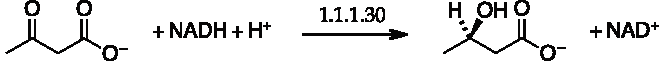
\includegraphics[scale=0.7]{images/HBDH_reaction1.pdf}
%  \caption[][5mm]{The building blocks of nylon-6 and nylon-6,6.} 
  \label{fig:react1}
\end{figure}

The rate of reaction was followed by measuring the change in NADH concentration using UV-vis spectrometry. This is a precise method and should give repeatable results.

\subsection{The Data}

Below are two sets of data from the publication (always check the supplement\-ary material for experimental details and data tables not presented in the publication.)

 
\begin{table}[h!]
    \caption[][0mm]{Michaelis-Menten turnover number, $k_{cat}$, vs. temperature for reaction of \textit{hydroxybutyrate dehydrogenase} with 3-oxobutanoate and 3-oxopentanoate.\\ \vspace{2mm} Data taken from tables S-1 and S-3 of the supplementary material for the the paper.\textsuperscript{\ref{paper1}} }

%    \sisetup{separate-uncertainty=true}
    \centering
    \fontfamily{ppl}\selectfont
    \begin{tabular}{
       S
       S[
               table-number-alignment = right,
                separate-uncertainty = true,
                table-figures-uncertainty = 1,
               table-figures-decimal = 1
        ]
       S[
                table-number-alignment = left,
                separate-uncertainty = true,
                table-figures-uncertainty = 1,
                table-figures-decimal = 1
        ]
       S[
               table-number-alignment = right,
                separate-uncertainty = true,
                table-figures-uncertainty = 1,
               table-figures-decimal = 1
        ]
       S[
                table-number-alignment = left,
                separate-uncertainty = true,
                table-figures-uncertainty = 1,
                table-figures-decimal = 1
        ]
        }
       % \toprule
             &  \multicolumn{4}{c}{$k_{cat}$ / \unit{\per\second}}  \\
           \cmidrule(lr){2-5} 
{Temp. (/ $K$)}  & \multicolumn{2}{c}{3-oxobutanoate}  & \multicolumn{2}{c}{3-oxopentanoate}  \\

\midrule
283  &     3.4  &\pm  0.1  &   0.21 &\pm 0.01  \\                
288  &     5.3  &\pm  0.2  &   0.28 &\pm 0.01  \\                 
293  &     7.6  &\pm  0.2  &   0.46 &\pm 0.02  \\                 
298  &     11.7 &\pm 0.3   &  0.60  &\pm 0.03  \\
303  &     15.2 &\pm 0.1   &  1.16  &\pm 0.02  \\
308  &     21.3 &\pm 0.9   &  1.47  &\pm 0.03  \\
313  &     27.8 &\pm 0.9   &  2.07  &\pm 0.09  \\
318  &     39   &\pm   3   &    2.7 &\pm  0.1  \\ 
323  &     52   &\pm   4   &    4.1 &\pm  0.2  \\ 
325  &     61   &\pm   2   &        &          \\  
328  &     69   &\pm   3   &    6.1 &\pm  0.4  \\ 
330  &     79   &\pm   7   &    6.6 &\pm  0.9  \\                             
        %\bottomrule
    \end{tabular}
    \label{tab:BzClSolv}
\end{table}


\clearpage

\section{Your Challenge}

Complete the following activities.

\begin{enumerate}
\item Construct an Eyring plot using the data above and perform a linear curve fit. Then complete the following activities.

\begin{enumerate}
\item Perform the curve fit with and without consideration of the estimated experimental errors. When using the experimental error, present error bars on the plots. How did you include the error from the rate data in your curve fit?

\item Report the slope and intercept, their respective standard deviation and the squared Pearson correlation constant ($r^2$). Why are these parameters slightly different when we do or do not include the exp\-er\-i\-ment\-al errors?

\item How do you think the errors were determined in these data sets?

\item Calculate the values for $\Delta H^\ddagger$ and $\Delta S^\ddagger$ with error-propagation.\sidenote
[][-20mm]{Error propagation for the Erying equation is expressed using the following two relationships:\\ \vspace{2mm}
$$ \sigma_{\Delta H^\ddagger} = \sqrt{2 \frac{R^2 T_{max}^2 T_{min}^2}{\left( T_{max}-T_{min}\right)^2} \left(\frac{\sigma_{k_{cat}}}{k_{cat}}\right)^2}$$

$$ \sigma_{\Delta S^\ddagger} = \sqrt{\frac{R^2 \left(T_{max}^2 + T_{min}^2\right)}{\left( T_{max}-T_{min}\right)^2} \left(\frac{\sigma_{k_{cat}}}{k_{cat}}\right)^2}$$ \vspace{2mm}}\sidenote
[][0mm]{Error propagation formula adapted from ``A Static Agostic \ce{\alpha-CH\cdots M} Interaction Observable by NMR Spectroscopy: Synthesis of the Chromium(II) Alkyl \ce{[Cr2(CH2SiMe3)6]^2-} and Its Conversion to the Unusual `Windowpane' Bis(metallacycle) Complex \ce{[Cr(\kappa^2-C,C$^\prime$-CH2SiMe2CH2)2]^2-}.'' P.M. Morse et al., \textit{Organometallics}, \textbf{1994}, \textit{13}, 1646-1655. \url{https://doi.org/10.1021/om00017a023}\vspace{2mm}}
Com\-ment on the precision of each parameter. The $r^2$ value was great; why is the precision so poor? Compare your results with the results of the authors. Comment on any differences.

\item Present the Erying plot with the $x$-axis starting from the origin (zero). Does that image provide any insight into the ?

\item Using the calculated activation parameters, predict value of $k_{cat}$ at a selected temperature. Using error-propagation, determine the estimated standard deviation for your results. How was the precision for this value?

\item Most Erying plots in the literature use four or five data points. Select any four data points from the sets above and repeat the above exercises. What happened to your precision when using less data?

\end{enumerate}

\item Linearizing mathematical models for the convenience of using linear re\-gres\-sion analysis is very 1980's.\sidenote
[][-0mm]{Without a doubt, the `80's was the greatest decade -- except for the computers. I miss my Commodore~64, but my current computer is one million times more powerful in every metric: 64~kilobytes vs. 16~gigabytes; no storage (or whatever an audio cassette tape could hold) vs. one terabyte; 4528~transistors vs. 16~million transistors; \qty{1.5}{MHz} vs. \qty{3.2}{GHz}; dial-up bulletin-board services using \qty{54}{kb/s} modems vs. the internet over optical fibre at \qty{300}{mb/s}. 

We have enormous computing power at our fingertips now. Why do we stick with methods meant for graph paper?} Perhaps we could try fitting the data directly to $k_{cat}$ vs. $T$ using non-linear curve fitting? Repeat the exercises described above. How is the precision now?

\item Document your methods for creating the plots, performing the curve fits and performing calculations with correct error-propagation. Explain how your method of documentation provides an unambiguous description of your math and methods. Does your documentation provide a tool that can be easily reused by yourself or your lab-mates in analyzing other sets of rate data at different temperatures?

\item Where in this process did Microsoft Excel become useless to you?

\end{enumerate}


\section{The Seminar}

In the seminar supported by this document we will introduce the following ideas:

\begin{enumerate}

\item We all love spreadsheets, but have we outgrown them?

\item \textit{Python} as a tool for data analysis. As an example, we will use the Erying plot data described above and explore the following concepts:

\begin{enumerate}

\item Linearized plots and their strengths and weaknesses.
\item Handling error propagation for strongly correlated parameters (e.g. when small changes in slope have an outsized effect on the intercept.)
\item Fitting the non-linear model of the Erying equation to your data.
\item Graphical approaches to expressing confidence intervals in your plots.

\end{enumerate}

\item Using \textit{Jupyter} notebooks as a method for using these \textit{Python} tools and providing documentation of your methods and reasoning. Allow others to read your code and read your mind.\sidenote[][-5mm]{Won't it be great to be able to figure out exactly what you were thinking when you did that thing that time.}

\end{enumerate}


\section{The Workshop}

In the workshop that will follow the seminar, participants will gain hands-on experience in the following:

\begin{enumerate}

\item Setting up \textit{Python} tools on your own computer. 

\begin{enumerate}

\item The \textit{Anaconda} package and its tools

\item Accessing the terminal and using terminal commands

\item Installing \textit{Python} modules using the \texttt{conda} command

\end{enumerate}

\item Using a \textit{Jupyter} notebook with interactive \textit{Python}

\begin{enumerate}

\item A notebook as a calculator

\item A notebook as a self-documenting and reusable data analysis tool

\item Exporting plots for use in your thesis and in publications.

\end{enumerate}

\item An overview of some useful \textit{Python} tools

\begin{itemize}
\item \texttt{uncertainties} --- error analysis
\item \texttt{numpy} --- all the math you will every need
\item \texttt{pandas} --- tabular data
\item \texttt{scipy} --- numerical methods and statistical analysis
\item \texttt{sympy} --- symbolic math
\item \texttt{matplotlib} --- professional plotting
\item \texttt{lmfit} --- an advanced curve fitting tool 

\end{itemize}

\end{enumerate}



\nobibliography{}

\end{document}